\section{Architettura}

\subsection{Introduzione}
Per la Realizzazione delle 3 webapp è stata adottata un architettura a microservizi, separando le funzioni di back-end da quelle del front-end. I vari microservizi di ciascuna webapp sono stati sviluppati su container docker differenti.
\subsubsection{Container Front-end}
\begin{itemize}
    \item \textbf{originIssuer:} È la componete di front-end della webapp Issuer. Essa si interfaccia con l'utente per inviare segnali e ricevere dati dal Back-end \textit{originIssuerApi}. Per la realizzazione del codice è stato adottato il pattern architetturale MVVM (Model-View-ViewModel).
    \item \textbf{originWallet:} È la componete di front-end della webapp Wallet. Essa si interfaccia con l'utente per inviare segnali e ricevere dati dal Back-end \textit{originWalletApi}. Per la realizzazione del codice è stato adottato il pattern architetturale MVVM (Model-View-ViewModel).
    \item \textbf{originVerifier:}È la componete di front-end della webapp Verifier. Essa si interfaccia con l'utente per inviare segnali e ricevere dati dal Back-end \textit{originVerfierApi}. Per la realizzazione del codice è stato adottato il pattern architetturale MVVM (Model-View-ViewModel).
\end{itemize}

\subsubsection{Container Back-end}
\begin{itemize}
    \item \textbf{originIssuerApi:} È la componente di back-end della webapp Issuer che si occupa di gestire le richieste provenienti dal front-end e di comunicare con il database \textit{originIssuerDB} per la memorizzazione dei dati.
    \item \textbf{originWalletApi:} È la componente di back-end della webapp Wallet che si occupa di gestire le richieste provenienti dal front-end e di comunicare con il database \textit{originWalletDB} per la memorizzazione dei dati.
\end{itemize}

\subsubsection{Container database}
\begin{itemize}
    \item \textbf{originIssuerDB:} È la componente della webapp Issuer che va a eseguire operazioni sul database per la richiesta e la memorizzazione di dati. 
    \item \textbf{originWalletDB:} È la componente della webapp Wallet che va a eseguire operazioni sul database per la richiesta e la memorizzazione di dati.
\end{itemize}

\subsubsection{Conteiner WaltId per strandard openID}
\begin{itemize}
    \item \textbf{openIdIssuer:} È una componente della libreria WaltID per mantenere lo standard openId di comunicazione tra Issuer e le altre webapp, al fine di rispettare le richieste del capitolato.
    \item \textbf{openIdWallet:} È una componente della libreria WaltID per mantenere lo standard openId di comunicazione tra Wallet e le altre webapp, al fine di rispettare le richieste del capitolato.
    \item \textbf{openIdVerifier:}È una componente della libreria WaltID per mantenere lo standard openId di comunicazione tra Verifier e le altre webapp, al fine di rispettare le richieste del capitolato.
\end{itemize}
 
\subsubsection{Container di supporto}
\begin{itemize}
    \item \textbf{adminer:} È un container che permette agli sviluppatori di gestire il database tramite interfaccia web.
    \item \textbf{nginx:} Lo utilizziamo come server proxy per gestire il reindirezzamento del traffico http tramite domini verso i container interni della rete docker
\end{itemize}






\subsection{Componenti Back-end}
\subsubsection{OriginiIssuerApi}
\begin{itemize}
    \item \textbf{authentication:}È una classe che si occupa della autenticazione, ovvero: login, registrazione. 
    \item \textbf{datasScrapper:}È un insieme di classi che si occupa di dialogare con il database reperendo e memorizzando i dati da esso. È stato realizzato tramite un insieme di 3 classi che rispettano il pattern strategy. 
    \item \textbf{openid:}È la classe che si occupa di comunicare con il container openIdIssuer. Essendo le chiamate dipendenti strettamente dallo sviluppo della libreria waltId, il gruppo ha preferito far comunicare il front-end non direttamente con la libreria waltId ma dialogare con questo layer intermedio. In questa maniera il backend si occuperà di fare le chiamate con la libreria waltId del container openIdIssuer.
    \item \textbf{DataResponse:}È una classe che si occupa di parametrizzare il tipo di ritorno che il backend fornisce.
    \item \textbf{InputChecker:}Contiene dei metodi necessari per la verifica e la correttezza degli input fatti al backend.
    \item \textbf{QRCodeGenerator:}È una classe fondamentale nel processo di credential issuing. Vi sono 2 modi per generare una credenziale ovvero: cros device e same device. Questa classe si occupa di generare un qrcode senza generare direttamente l'immagine ma dando via risorsa al frontend lo stream dell'immagine del qrcode tramite il metodo \textit{pipeGenerateQR}.
    \item \textbf{Routing:} In questa classe vengono definite 2 funzionalità principali:
     \begin{itemize}
     \item Cors ovvero una funzionalità per limitare l'uso da altri dispositivi. Questa opzione viene configuarata tramite corsOptions specificando gli indirizzi di origine da cui un utilizzatore potrà usare il backend. 
     \item Express è una funzionalità che permette di offrire degli endpoint con cui un altro applicativo potrà fare delle chiamate http. 
     \end{itemize}
    Nel componente vengono configurate le nostre classi precedentemente elencate.
    Inoltre la clsse specifica tutte le chiamate possibili del backend originIssuerApi.

    
    \item \textbf{index:}Viene creato il routing e il metodo di configurazione degli endpoint.
\end{itemize}
\subsubsection{OriginWalletApi}
\begin{itemize}
    \item \textbf{authentication:}È una classe che si occupa della autenticazione, ovvero: login, registrazione. 
    \item \textbf{datasScrapper:}È un insieme di classi che si occupa di dialogare con il database reperendo e memorizzando i dati da esso. È stato realizzato tramite un insieme di 3 classi che rispettano il pattern strategy. Essendo il database del Walle irrisorio si potrebbe usare un ulteriore strategia, memorizzando i dati su un file XML o JSON. Questo poichè la struttura dei dati e la complessità è semplice e senza relazioni particolari.
    \item \textbf{openid:}È la classe che si occupa di comunicare con il container openIdWallet. Essendo le chiamate dipendenti strettamente dallo sviluppo della libreria waltId, il gruppo ha preferito far comunicare il front-end non direttamente con la libreria waltId ma dialogare con questo layer intermedio. In questa maniera il backend si occuperà di fare le chiamate con la libreria waltId del container openIdWallet.
    \item \textbf{DataResponse:}È una classe che si occupa di parametrizzare il tipo di ritorno che il backend fornisce.
    \item \textbf{InputChecker:}Contiene dei metodi necessari per la verifica e la correttezza degli input fatti al backend.
    \item \textbf{Routing:} In questa classe vengono definite 2 funzionalità principali:
    \begin{itemize}
    \item Cors ovvero una funzionalità per limitare l'uso da altri dispositivi. Questa opzione viene configuarata tramite corsOptions specificando gli indirizzi di origine da cui un utilizzatore potrà usare il backend. 
    \item Express è una funzionalità che permette di offrire degli endpoint con cui un altro applicativo potrà fare delle chiamate http. 
    \end{itemize}
    Nel componente vengono configurate le nostre classi precedentemente elencate.
    Inoltre la clsse specifica tutte le chiamate possibili del backend originIssuerApi.
\end{itemize}

\subsection{Componenti Front-end}
\subsubsection{originIssuer} 
\begin{itemize}
    \item 
\end{itemize}
\subsubsection{originWallet}
\begin{itemize}
    \item \textbf{App:} questa è la pagina iniziale dell'applicazione, dove viene definito il \textit{routing} delle pagine.
    \item \textbf{components/Navbar:} questa è la componente che definisce la \textit{navbar} dell'applicazione, che differisce dal tipo di utente che è loggato (user, guest, ...).
    \item \textbf{controller/LoginController:} questa è la componente che gestisce la pagina di login dell'applicazione. Esso crea la corrispondente 
    \textit{LoginViewModel} e la corrispondente \textit{LoginView}. Il \textit{controller} si occupa di gestire gli eventi provenienti 
    dalla \textit{view} e di aggiornare la \textit{viewModel}, che a sua volta aggiorna il \textit{model} presente nel back-end.
    \item \textbf{controller/LoginViewModel:} Viene creato dal \textit{controller} ma non ha nessun riferimento ad esso, posside solo il riferimento al modello dei dati che esso posside.
    \item \textbf{controller/LoginView:} viene creato dal \textit{controller} ma non ha nessun riferimento ad esso, posside solo il riferimento al modello dei dati che esso posside e qualche indicazione di \textit{handling} dei dati.
    \item \textbf{ViewModel:} componente che si occupa del collegamento con il back-end, ha quindi un riferimento al \textit{model}. È unico per tutta l'applicazione\\
    \\NB. Tutte le componenti seguono la struttura MVVM sopra descritta per la componente \textit{Login}.
    \item \textbf{ListCredential:} componente che si occupa di mostrare la lista delle credenziali dell'utente presenti nel \textit{Wallet}. Da qui si può andare nel dettaglio di una singola credenziale.
    \item \textbf{DetailCredential:} componente che si occupa di mostrare i dettagli di una credenziale presente nel \textit{Wallet}. Da qui si può eliminare una credenziale.\\
    \\NB. Le seguenti componenti hanno nomi controintuitivi ma sono imposti dallo standard \textit{openID}.
    \item \textbf{InitiateIssuance:} componete che si  occupa dell'accettazione di una richiesta di credenziale da parte di un \textit{Issuer} e vengo reindirizzato alla pagina \textit{ListCredential}.
    \item \textbf{CredentialRequest:} Componente che si occupa del re indirizzamento di una richiesta di presentazione di una credenziale parte del \textit{Verifier}. 
\end{itemize}
\subsubsection{originVerifier}

\subsection{Componenti database}
\begin{itemize}
    \item \textbf{originIssuerDB:}\\
    \begin{center}
        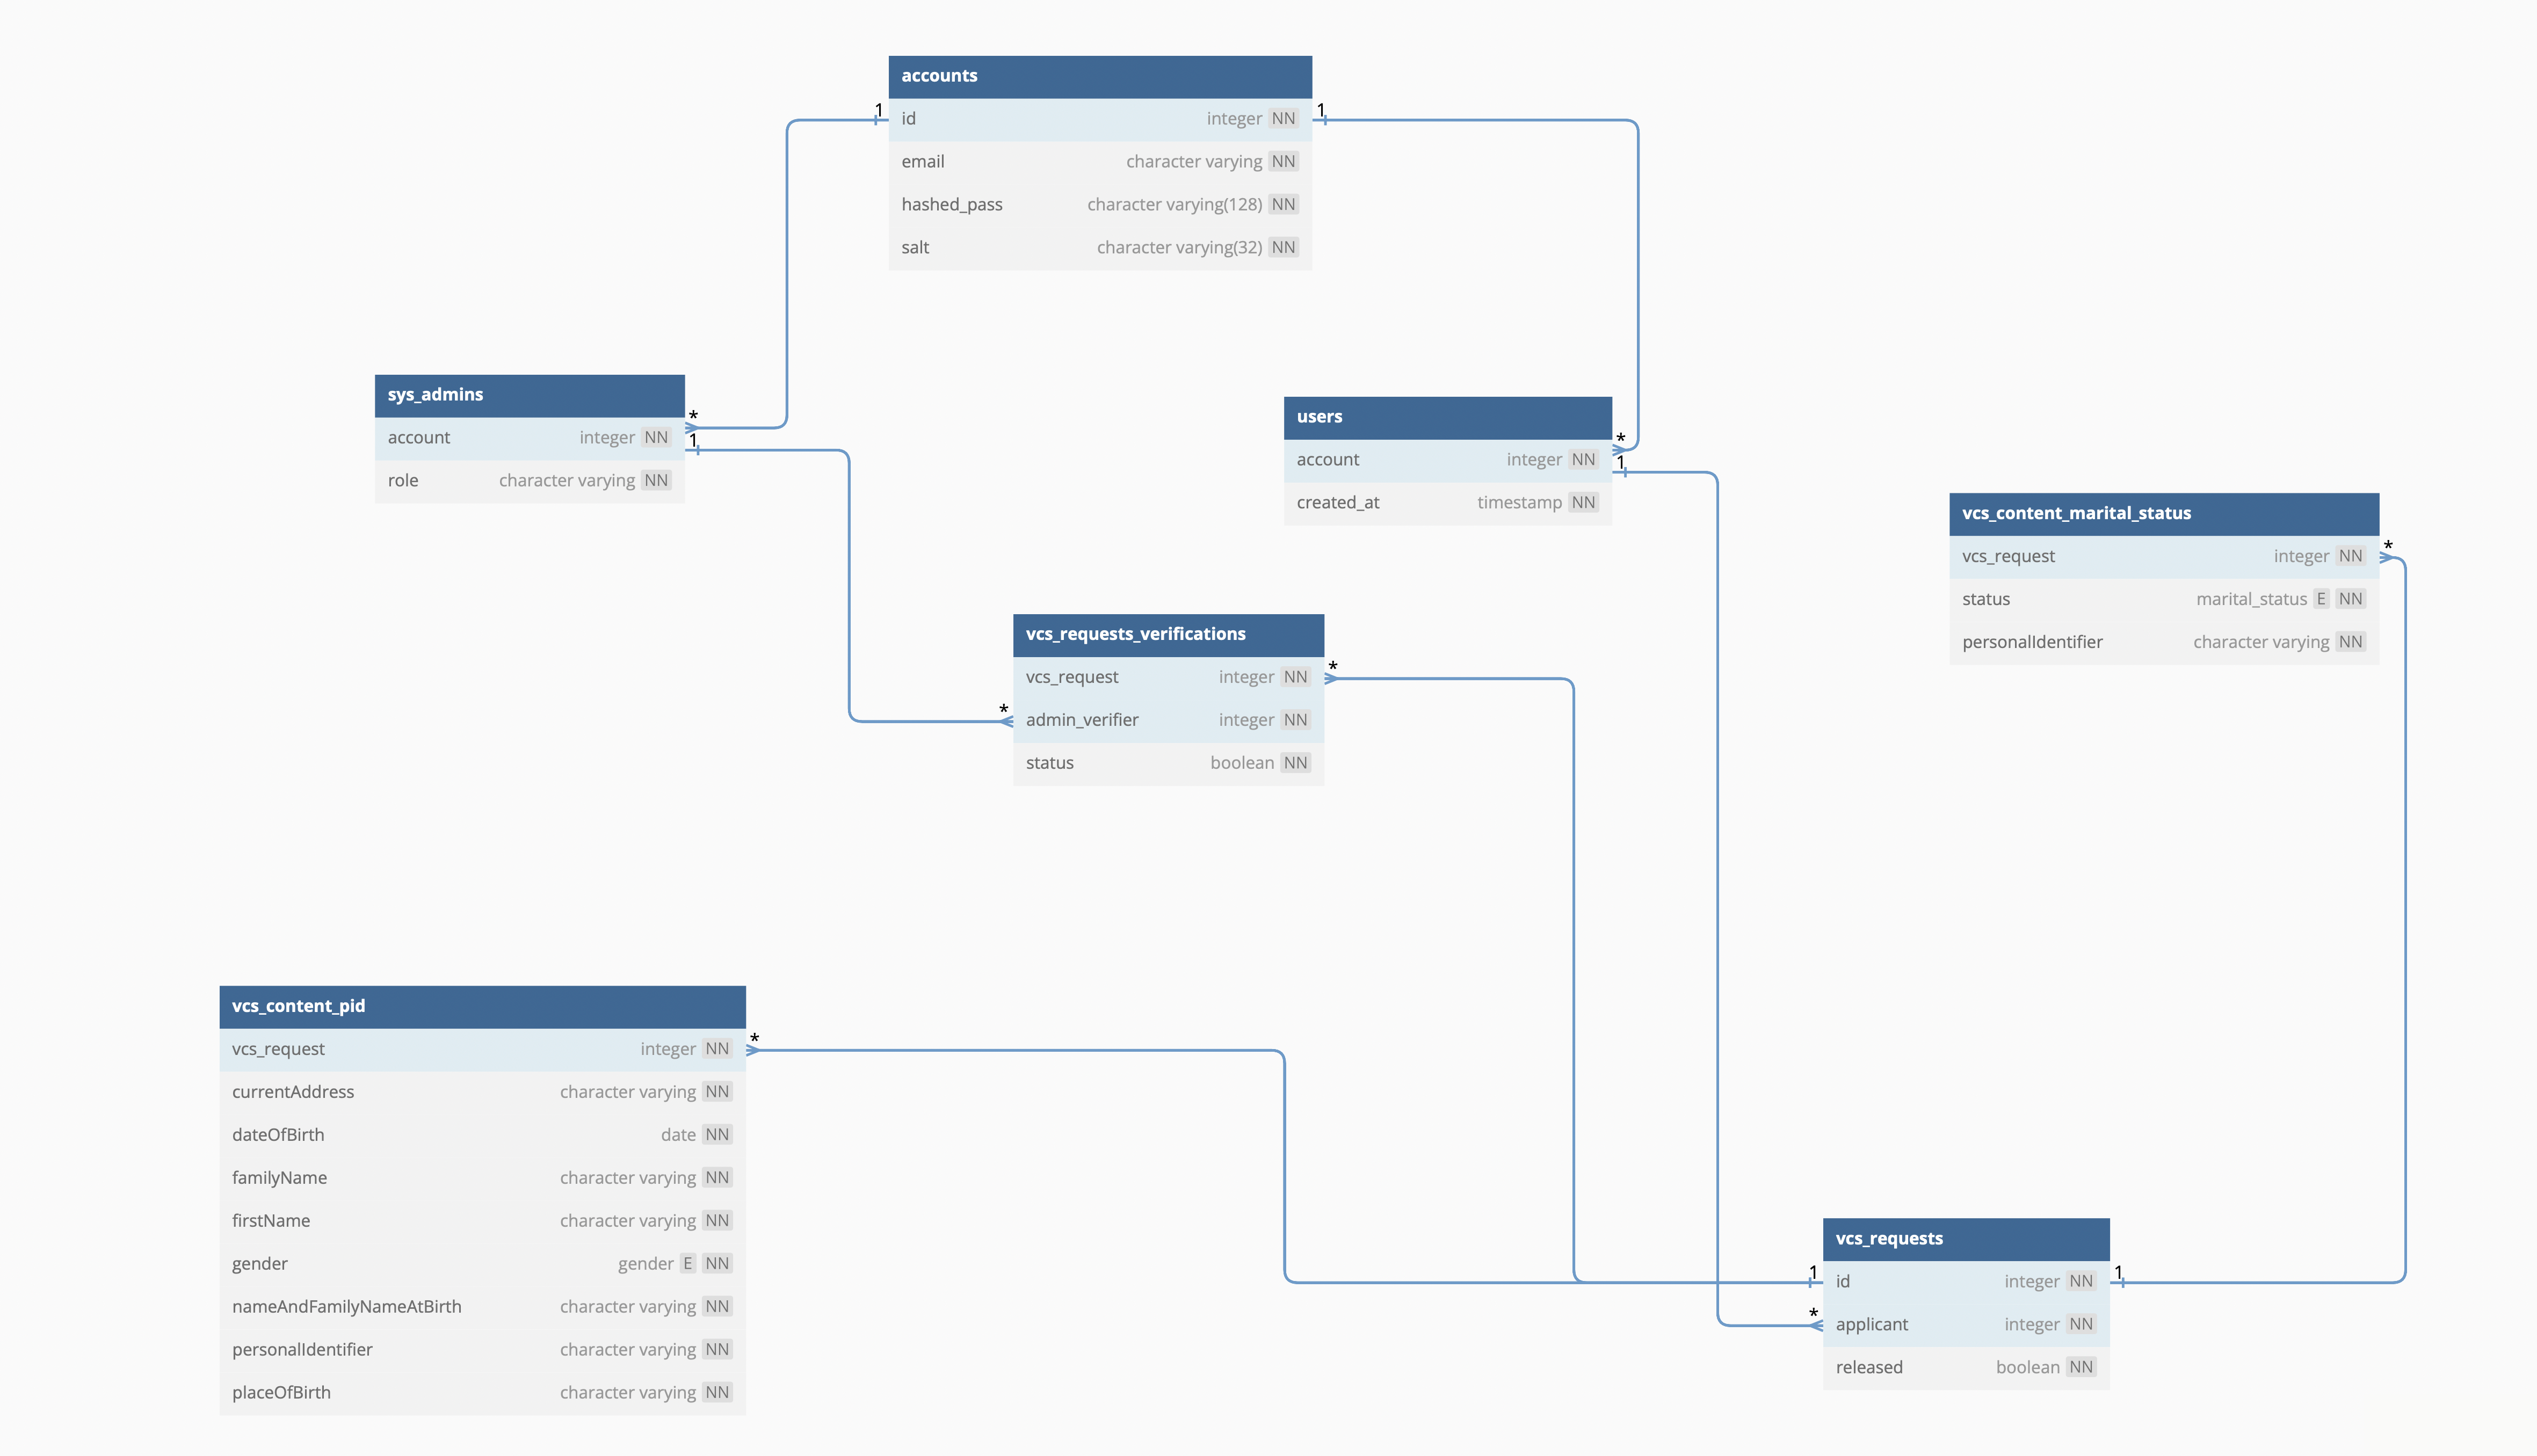
\includegraphics[scale = 0.3]{./res/img/issuerdb.png}
      \end{center}
    L'immagine sopra riportata descrive il database "issuerdb" implementato mediante un grafico entità-relazioni (schema ER).\\
    Issuerdb è stato pensato per gestire e conservare le informazioni legate agli utenti, alle richieste di certificati digitali (VCS requests) e alle verifiche dei certificati stessi.
    Per quanto richiesto dal capitolato, e per rispettare la logica dietro tutto il meccanismo dell'Issuer, si distinguono 2 tipi diversi di account: gli account "sys\_admins" e gli account "users".\\
    \begin{itemize}
    \item "sys\_admins" sono gli account utilizzati dagli amministratori di sistema, cioè quelle entità che si occupano di approvare (o meglio, verificare) le richieste degli "users" (VCS requests).\\
    \item "users", invece, sono gli account utilizzati dai semplici utilizzatori del servizio. Si occupano semplicemente di effettuare delle richieste di certificati di loro interesse alle entità che si occupano di verificare i certificati.\\
    \end{itemize}
    Il contenuto della richiesta approvata e rilasciata può essere di 2 tipi soltanto: un "vcs\_content\_marital\_status" (contenuto riferito allo stato di matrimonio di un utente) o un "vcs\_content\_pid" (contenuto riferito ad un documento PID di un utente).\\




    \item \textbf{originWalletDB:}
     \begin{center}
        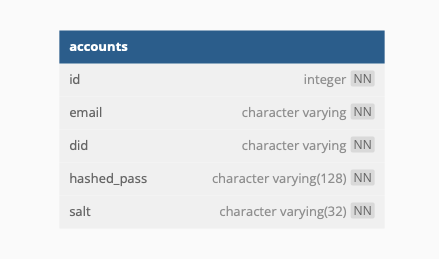
\includegraphics[scale = 0.6]{./res/img/walletdb.png}
      \end{center}
    
    L’immagine sopra riportata descrive il database “walletdb” implementato mediante un grafico entità-relazioni (schema ER).
    Walletdb è stato pensato per gestire e conservare (fare lo “storing”) le informazioni legate alle credenziali degli utenti, come espresso da capitolato.\\
    
\end{itemize} 


\subsection{Diagramma delle classi}

\subsection{Design pattern}
\paragraph{Strategy}:
\paragraph{Model View-ViewModel}
